\subsection{Gradient Boosting}\label{subsec:grad_boost}


The following section is based on \cite{Chen16} and \cite{Murphy}. 

Gradient boosting is about iteratively generating a set of gradient trees that solve a given classification problem as effectively as possible.

Gradient trees are essentially decision trees, except that each leaf of the tree  has a value (weight) $w_i \in \R$ assigned to it. Consequently, a gradient tree with $T$ leaves and corresponding weights $\{w_1, ... ,w_T\}$ can be understood as a function $f: \R^m \to \R$ . Each data point $x \in \R^m$ is assigned the weight of the leaf corresponding to $x$ by $f$ via $f(x) = w_{q(x)}$. The function $q: \R^m \to T$ assigns a sample $x$ to the index number of the leaf belonging to $x$. Furthermore $I_j := \{ i \mid x_i \in q^{-1}(j) \}$ contains the indices of those samples which refer to the leaf number $j$. The set of all gradient trees is called $\mathcal{F}$. \todo{holprig?}

\begin{minipage}{.45\linewidth}
	\begin{figure}[H]
		\begin{center}
			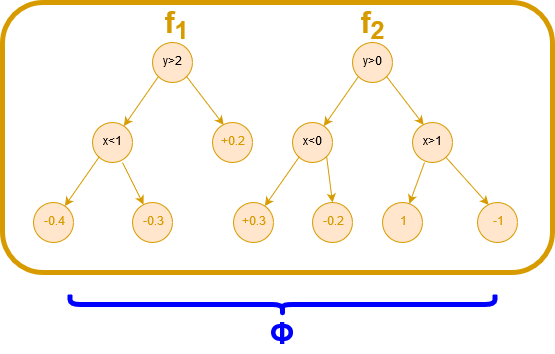
\includegraphics[width=\linewidth]{images/gradient_trees_example.png}
		\end{center}		
	\end{figure}
\end{minipage}
\hfill
\begin{minipage}{.5\linewidth}
	A tree ensemble model $\{f_1, ... ,f_K \mid f_i \in \mathcal{F}\}$ consisting of $K$ gradient trees is not evaluated by voting, as known from decision trees, but by adding the function values of the sample $x$ of the single gradient trees in the ensemble function $\Phi = \sum f_k$. The predicted outcome $\hat{y}$ of a sample $x$ results from this:
\end{minipage}

$$\hat{y} = \Phi(x) = \sum_{k=1}^{K} f_k(x)$$

Given a sample set $X= \{x_1, ..., x_n\} \subset \R^{m} $ of $n$ samples each with $m$ features and the corresponding ground truths $\{y_1, ... ,y_n\}$, the resulting regularization function is found in:	
$$\mathcal{L} = \sum_{i=1}^{n} l(y_i, \Phi(x)) + \sum_{k=1}^{K}\Omega(f_k) \text{,  where } \Omega(f_k) = \gamma T + \frac{1}{2}\lambda \norm{w}_2^2$$
$l$ is the loss-function, a convex function that is differentiable several times. $\Omega$ is a penalizing term in this context and monitors the structure of the tree within $\LL$. The choice of $\gamma$ influences the number of permissible leaves and $\lambda$ influences their weights. Thus $\Omega$ is a preventive measure against overfitting. Consequently, the model created with $\LL$ prefers gradient trees of simple shape.

\begin{figure}[H]
	\begin{center}
		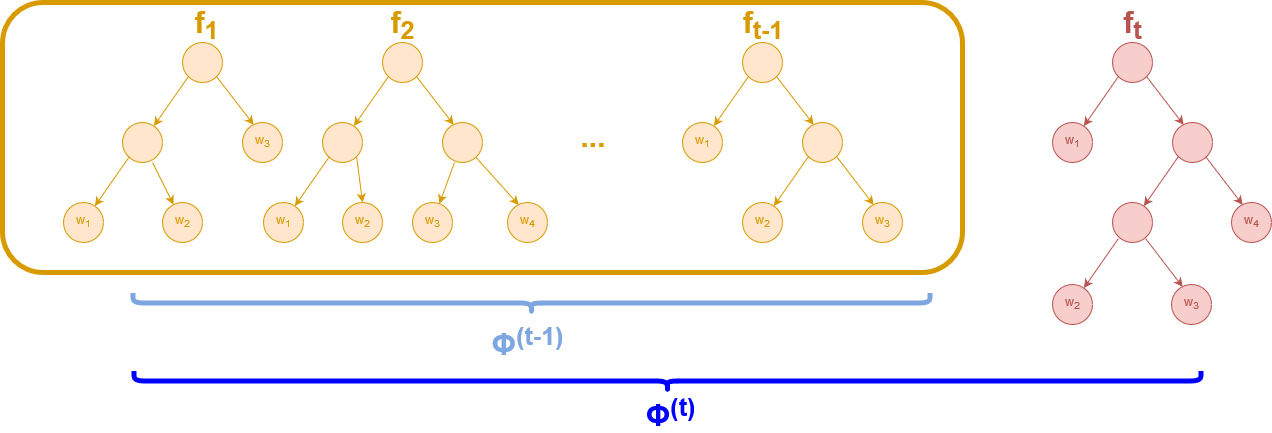
\includegraphics[width=\textwidth]{images/gradient_boosting.png}
		\caption{Visualisation of the $t$-th iteration step: For a fixed tree $f_t$ its weights $w_i$ have to be optimized with respect to the already existing set of trees.}
		\label{abb:gradient_boosting}
	\end{center}		
\end{figure}
The actual gradient tree boosting takes place by iteratively adding new trees to the ensemble. In the $t$-th iteration step, the ensemble consists of the gradient trees $\{f_1, ... , f_{t-1}\}$ created in the previous steps. The goal is to select the new gradient tree $f_t$ so that it improves the current model the most. This is the case if and only if 
\begin{equation}
\LL^{(t)} = \sum_{i=1}^{n} l(y_i, \Phi(x_i)) + \sum_{k=1}^{K}\Omega(f_k)
\label{eq:LL1}
\end{equation}
is minimized. Since the $\Omega(f_k)$ for the trees $f_1, ... f_{t-1}$\todo{caption oben} are already fixed, they can be omitted from here on. Furthermore, the first $t-1$ terms of the sum $\Phi(x_i) = f_1(x_i) + ... + f_{t-1}(x_i) + f_t(x_i)$ are already established in the $t$-th iteration. This sum is constant and aggregated in the expression $\hat{y}^{t-1}$, since it represents the predicted outcome after the $(t-1)$-th iteration step of the ensemble.

With this, (\ref{eq:LL1}) can also be formulated as:
\begin{equation}
\LL^{(t)} = \sum_{i=1}^{n} l(y_i, \hat{y}^{(t-1)} + f_k(x_i)) + \Omega(f_t)
\label{eq:LL2}
\end{equation}

To separate the dependency of $l$ and $f_t$, the 1D-taylor series expansion is executed at the location $(y_i,\hat{y}^{(t-1)})$ on the function $l$ and in the second coordinate only. Although $l$ is a 2D function, changes in the context of $\LL$ only take place in one coordinate, which is why it is allowed to interpret it as a 1D function - like $l(y_i,x) = l_{y_i}(x)$. It follows:
\begin{equation}
\label{eq:taylor}
l_{y_i}(\hat{y}^{(t-1)} + f_k(x_i)) = l_{y_i}(\hat{y}^{(t-1)}) + l_{y_i}^{'}(\hat{y}^{(t-1)}) \cdot f_k(x_i)
+ \newline \frac{1}{2} l_{y_i}^{''}(\hat{y}^{(t-1)}) \cdot f_k(x_i)^2 + R_\text{taylor}
\end{equation}

For readability's sake we write $g_i = l_{y_i}^{'}(\hat{y}^{(t-1))}) ) = \frac{\partial l}{\partial \hat{y}^{(t-1)}}(y_i,\hat{y}^{(t-1)})$ and $h_i = l_{y_i}^{''}(\hat{y}^{(t-1)}) ) = \frac{\partial l}{\partial^2 \hat{y}^{(t-1)}}(y_i,\hat{y}^{(t-1)})$. $g_i$ and $h_i$ are constants, because both $y_i$ and $\hat{y}^{(t-1))}$ are known in the current iteration step. Applying the results from equation (\ref{eq:taylor}) to $\LL^{(t)}$ yields:
\begin{equation} \label{eq:shortL}
\LL^{(t)} \approx \sum_{i=1}^{n} (l(y_i,\hat{y}^{(t-1)}) + g_if_t(x_i) + \frac{1}{2} h_i f_t(x_i)^2) + \Omega(f_t)
\end{equation}

Since the constant terms $l(y_i,\hat{y}^{(t-1)})$ do not depend on $f_t$, they can be ignored in the optimization problem and the result is the simplified objective:
\begin{equation} \label{eq:LLeinfach}
\tilde{\LL}^{(t)} = \sum_{i=1}^{n}( g_if_t(x_i) + \frac{1}{2} h_i f_t(x_i)^2) + \Omega(f_t)
\end{equation}

This term can now be further simplified by writing out $\Omega(f_t) = \gamma T + \frac{1}{2}\lambda \sum_{j=1}^{T} w_j^2$. For a given tree structure $q$ we get the different $I_j$, which can be used to change the order of summation. For this, $f_t(x_i)$ is expressed as the corresponding weight $w_j$ of the new tree $f_t$. The rearrangement is done by sorting by the appearing $w_j$. Applied to (\ref{eq:LLeinfach}), this results in:
\begin{equation} \label{eq:LL_umsortiert}
\tilde{\LL}^{(t)} = \sum_{j=1}^T\left( (\sum_{i \in I_j} g_i) w_j + \frac{1}{2} (\sum_{i \in I_j} h_i + \lambda)w_j^2 \right) + \gamma T
\end{equation}

It should be noted that for this rearrangement and a concrete evaluation of the equation above a \textit{fixed} tree structure $q$ must be provided. This means that the tree must already be finalized - except for the weights of its leaves.

To find the optimal weights $w^*_j$ for this fixed structure of $f_t$, $\tilde{\LL}^{(t)}$ from equation (\ref{eq:LL_umsortiert}) is derived in the direction of the corresponding $w_j$ and it yields:
\begin{equation} \label{eq:LL_ableitung}
\frac{\partial \tilde{\LL}^{(t)}}{\partial w_j} = \sum_{i \in I_j} g_i + (\sum_{i \in I_j} h_i + \lambda)w_j
\end{equation}

By setting this equation to $0$ and solving it for $w_j$, the optimal $w^*_j$ are gained, which minimize $\tilde{\LL}^{(t)}$:
\begin{equation} \label{eq:opt_w}
w_j^* = - \frac{\sum_{i \in I_j} g_i}{\sum_{i \in I_j} h_i + \lambda}
\end{equation}

Using these optimal $w_j^*$ in (\ref{eq:LL_umsortiert}) results in the optimal value of $\tilde{\LL}^{(t)}$ for the beforehand fixed tree structure $q$:
\begin{equation} \label{eq:entropy}
\tilde{\LL}^{(t)} (q) = - \frac{1}{2} \sum_{j=1}^{T} \frac{(\sum_{i \in I_j} g_i)^2}{\sum_{i \in I_j} h_i + \lambda} + \gamma T
\end{equation}

For a given tree structure $q$, it is now possible to calculate the most helpful weights of the new tree $f_t$ for the ensemble using (\ref{eq:opt_w}). Furthermore, such an (optimized) tree structure $q$ can be evaluated with (\ref{eq:entropy}). The resulting value is comparable to the entropy of decision trees. 

In reality one would have to work through all possible tree structures, including the different feature-splits, calculate the optimized $w^*_j$ and $\tilde{\LL}^{(t)} (q)$, and compare. Because this is hardly realizable, the new tree $f_t$ is constructed in the iteration step $t$ by a greedy algorithm. In this process, branches are added iteratively to the tree by splitting leaves. Let $I_l, I_r$ be the sets of the index numbers assigned to the left or right leaf and $I = I_l \dot\cup I_r$ the index set of the former leaf. The resulting improvement of this split results after (\ref{eq:entropy}):
\begin{equation} \label{eq:LRsplit}
	\begin{split}
		\tilde{\LL}_\text{split} &= \tilde{\LL}^{(t)} (q_\text{alt})-\tilde{\LL}^{(t)} (q_\text{neu})\\
		&= \left( - \frac{1}{2} \sum_{j=1}^{T} \frac{(\sum\limits_{i \in I_{j, \text{alt}}} g_i)^2}{\sum\limits_{i \in I_{j, \text{neu}}} h_i + \lambda} + \gamma T \right)- \left( - \frac{1}{2} \sum_{j=1}^{T+1} \frac{(\sum\limits_{i \in I_{j, \text{neu}}} g_i)^2}{\sum\limits_{i \in I_{j, \text{neu}}} h_i + \lambda} + \gamma (T+1) \right)\\	
		&= \frac{1}{2} \left( \frac{(\sum_{i \in I_l} g_i)^2}{\sum_{i \in I_l} h_i + \lambda} + \frac{(\sum_{i \in I_r} g_i)^2}{\sum_{i \in I_r} h_i + \lambda} - \frac{(\sum_{i \in I} g_i)^2}{\sum_{i \in I} h_i + \lambda} \right) - \gamma 
	\end{split}
\end{equation}

The second equality follows from the fact that the index sets $I_j$ do not differ except for the split leaf, i.e. the index sets $I, I_l$ and $I_r$, and thus cancel each other out.


